\section{Experimental Evaluation}
In this section we experimentally evaluate  Crypt$\epsilon$ to assess its practical utility  based on two parameters, the accuracy and the performance of the Crypt$\epsilon$ programs. Specifically the experiments were designed to answer the following questions:
\begin{enumerate}\item Does Crypt$\epsilon$ programs have constant error bounds depending only on the privacy parameter $\epsilon$  which is at least $O(\sqrt{m})$ times lower than that for the corresponding state-of-the-art LDP implementation? \item Is the program execution timings for Crypt$\epsilon$ practical? \item Does the proposed DP- optimizations provide substantial performance improvement over the base case Crypt$\epsilon$ implementation? \end{enumerate}

\paragraph{Methodology:} To answer the aforementioned questions we ran the experiments on the 7 Crypt$\epsilon$ programs previously outlined in section 5. We ran our experiments on a dataset which is generated from the UCI Adult dataset by randomly sampling 1000 records. The experiment numbers are reported as the mean value after 10 repetitions.
\subsection{Accuracy}
\begin{figure*}
    \centering
    \begin{subfigure}[b]{0.2\textwidth}
        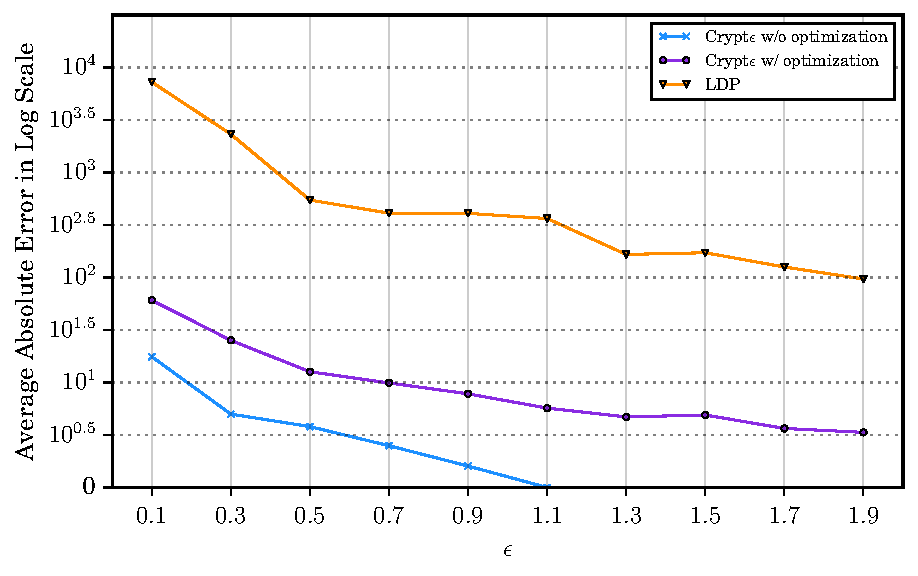
\includegraphics[width=5cm,height=5cm]{test1_1.pdf}
        \caption{ Program 1}
        \label{fig:gull}
    \end{subfigure}\quad \qquad\quad \\%
    ~ %add desired spacing between images, e. g. ~, \quad, \qquad etc.
      %(or a blank line to force the subfigure onto a new line)
    \begin{subfigure}[b]{0.3\textwidth}
       \qquad 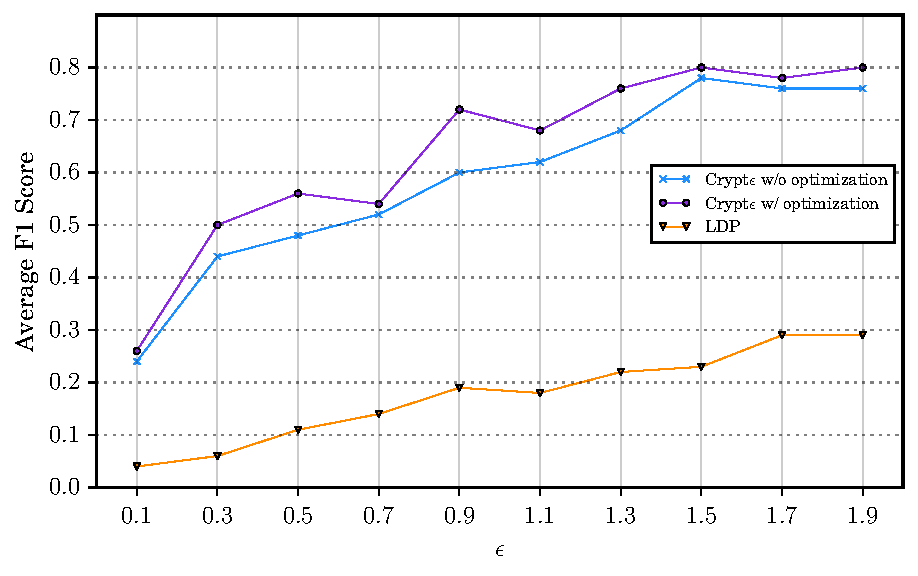
\includegraphics[width=5cm,height=5cm]{test2.pdf}
        \caption{ Program 2}
        \label{fig:tiger}
    \end{subfigure}
    ~ %add desired spacing between images, e. g. ~, \quad, \qquad etc.
      %(or a blank line to force the subfigure onto a new line)
    \begin{subfigure}[b]{0.3\textwidth}
    \qquad    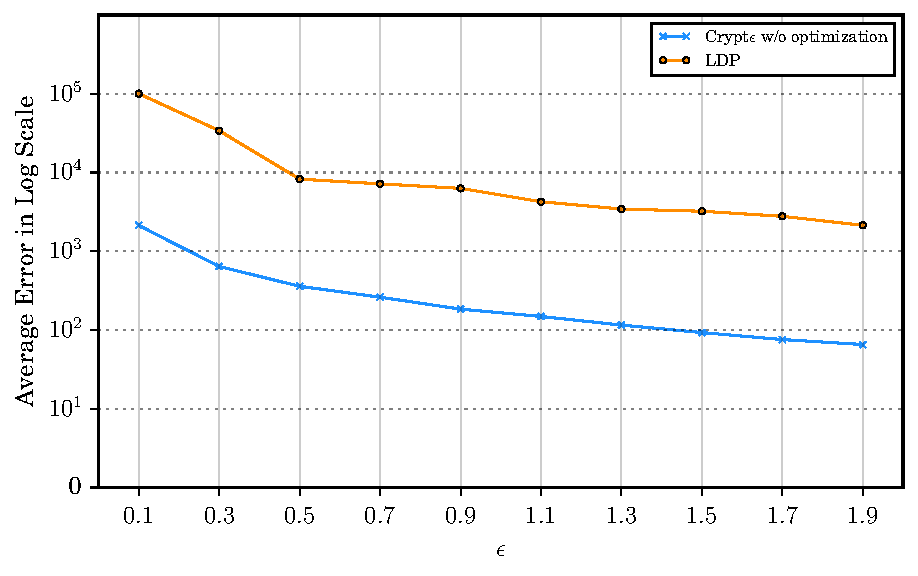
\includegraphics[width=5cm,height=5cm]{test3.pdf}
        \caption{Program 3}
        \label{fig:mouse}\end{subfigure}
          \begin{subfigure}[b]{0.3\textwidth}
    \qquad    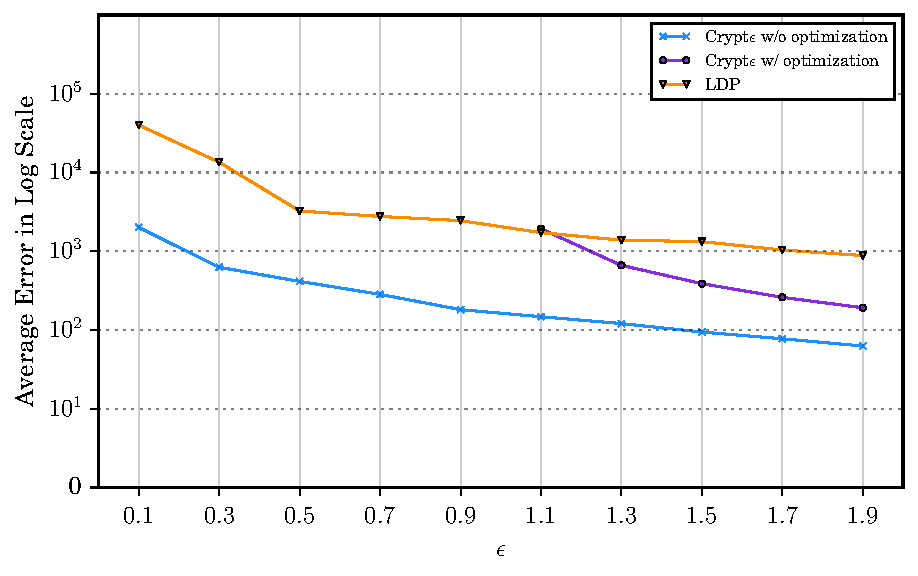
\includegraphics[width=5cm,height=5cm]{test4.pdf}
        \caption{Program 4}
        \label{fig:mouse}\end{subfigure}
          \begin{subfigure}[b]{0.3\textwidth}
    \qquad    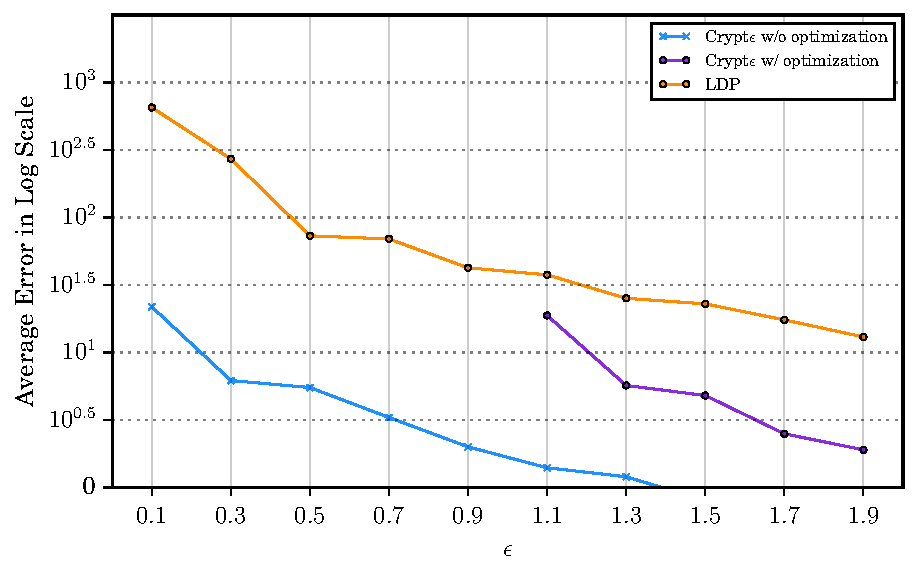
\includegraphics[width=5cm,height=5cm]{test55.pdf}
        \caption{Program 5}
        \label{fig:mouse}\end{subfigure}
          \begin{subfigure}[b]{0.3\textwidth}
    \qquad    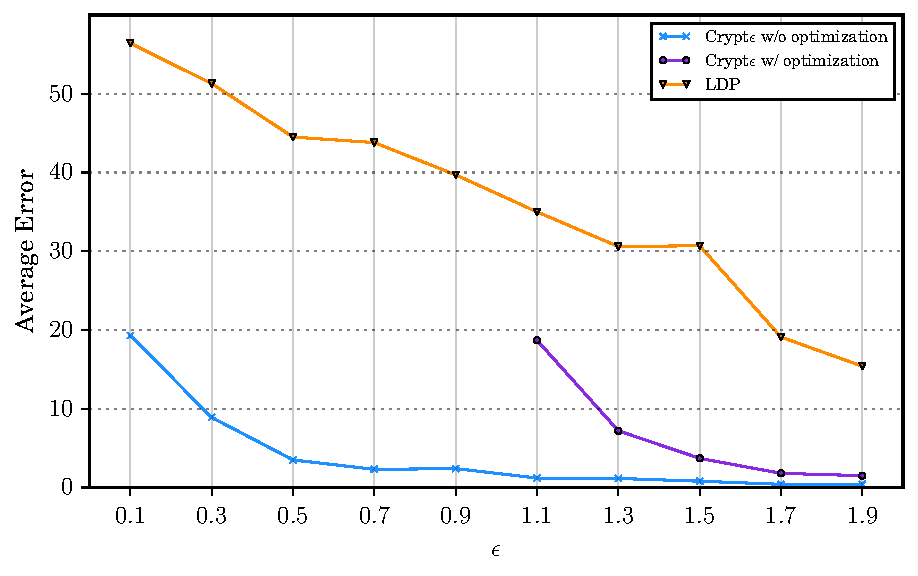
\includegraphics[width=5cm,height=5cm]{test66.pdf}
        \caption{Program 6}
        \label{fig:mouse}\end{subfigure}
          \begin{subfigure}[b]{0.3\textwidth}
    \qquad    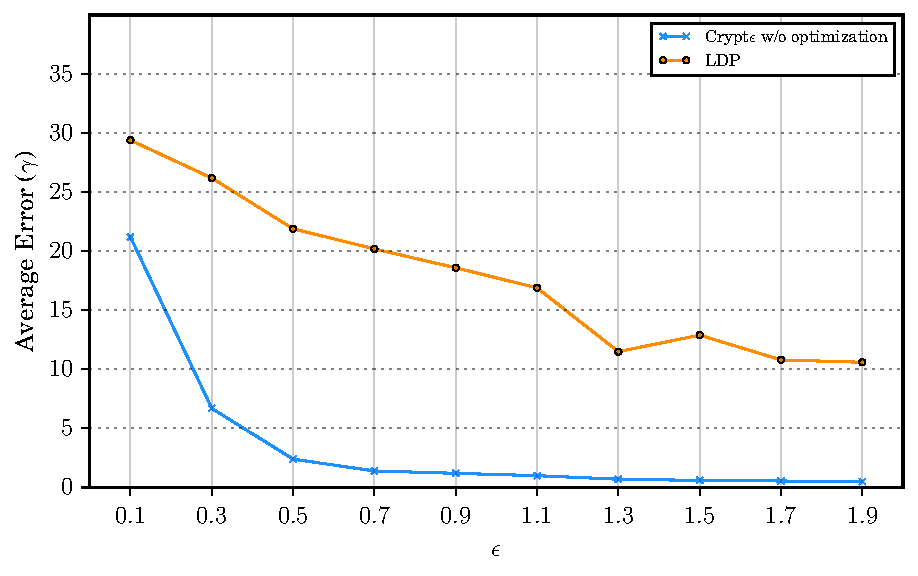
\includegraphics[width=5cm,height=5cm]{test7.pdf}
        \caption{Program 7}
        \label{fig:mouse}
    \end{subfigure}
%    \caption{a) External alignment is the neighborhood of read $X$ in the full genome and $\lambda$ is the \% of $X$ that correctly identifies it. (b) Internal alignment is the index-to-index alignment within the neighborhood of $X$ and $\sigma=avg_i\frac{TBScore_{opt}-TBScore_i}{TBScore_{opt}}$ where $TBScore_{i}=\sum_{[i,j] \in \textit{Traceback path}}\mathbf{M}[i,j]$. 
%   (c) $\rho$ is the number of reads required to cover a single index such that Pr( SNPs are aligned correctly in $Y) > 0.95$}
   \caption{Accuracy Analysis}
\end{figure*}
\subsection*{Crypt$\epsilon$ Program 1}
Program 1 counts the number of records having age in range [50,60].  
\\\textbf{\textsf{LDP} Competitor} - The competing \textsf{LDP} implementation uses the frequency oracle of \cite{LDP1}. 
\\\textbf{Error Measure} - The error measure used is  $Error = |C-\hat{C}|$ where $C$ is the true count and $\hat{C}$ is the noisy differentially private output. We report the mean error observed over 10 repetitions. \\
\textbf{Optimization}- For this program, the optimized implementation uses the range tree to answer the counting query.
\\\textbf{Observations} - For Program 1 we report our experimental results in Figure 3a. The first observation is that the error for the base case Crypt$\epsilon$ implementation is approximately $\frac{2}{\epsilon}$ (error=$17.60$ for $\epsilon=0.1$, mean error = $0.1$ for $\epsilon=1.9$). This is in cohorts with our expectation as we add two instances of Laplace noise at the \textsf{AS} and the \textsf{CSP} and s.t.d of $Lap(\frac{1}{\epsilon})$ is given by $\frac{1}{\epsilon}$. In contrast, the error corresponding to the $\textsf{LDP}$ implementation is at least $400 >11\cdot \sqrt{m}=  11\cdot \sqrt{1000} \approx 352$ times worse. This observation is intuitive as each frequency oracle count for the \textsf{LDP} is expected to have $O(\frac{\sqrt{m}}{\epsilon})$ error and for answering Program 1 we need to read $11$  such counts (for the range [50,60]). For e.g., the error for $\textsf{LDP}$ is $967 \times$  higher than that of Crypt$\epsilon$ for $\epsilon=1.9$. Another observation is that the accuracy of the range tree based Crypt$\epsilon$ implementation is poorer as compared to that of the base case. For e.g., for $\epsilon=0.3$, the error for the optimized implementation is $25.2$ while that for the base case is $5$. This is so because the sensitivity of the range tree is $\log k$ where $k$ is the number of leaves and a range query can take up to $2 \log k$ nodes for answering. Thus for a single query, the base case implementation will give better accuracy results. The accuracy gain for range trees kicks in for answering multiple range queries as showcased in Fig .  \arc{TO-DO New exp to showcase range tree accuracy gain}
\subsection*{Crypt$\epsilon$ Program 2}
Program 2 counts the top 5 most frequent age values.
\\\textbf{\textsf{LDP} Competitor} - The competing \textsf{LDP} implementation uses the frequency oracle of \cite{LDP1}. 
\\\textbf{Error Measure} - The error measure used is given by $\sigma= \text{the fraction of age values }$ returned in the top 5 that have value less than $ct_5-\alpha$  where  $ct_5$ is the count of the $5^{th}$ largest value and $\alpha=\frac{1}{\epsilon}\log\frac{1}{\delta}$ is a slack parameter. The slack parameter is required because with probability $1-\delta$ no differentially private algorithm can distinguish between any two counts that differ by less than $\alpha$. \\
\textbf{Optimization}- The optimized implementation reads of the values of all the leaves in  the range tree (each leaf corresponds to the count of a single age value) and returns age values with the top 5 counts.
\\\textbf{Observations} - The experimental results of  Program  2 are reported in  Figure 3b. 

\subsection*{Crypt$\epsilon$ Program 3}
Program 3 reports the marginal on attributes \textsf{Age} and \textsf{Gender}.  
\\\textbf{\textsf{LDP} Competitor} - For the  \textsf{LDP} implementation, we construct a frequency oracle based on \cite{LDP1} over the marginal attribute $\textsf{Age}\times\textsf{Gender}$. 
\\\textbf{Error Measure} - For Program 3 we use the L1-norm error metric $ Error=\sum_{i}|C[i]-\hat{C}[i]|, i \in [200]$ where $C$ is the true marginal and $\hat{C}$ is the noisy one. 
\\\textbf{Observations} - Figure 2c reports the experimental results for Program 3. Attribute $Age$ has domain size $100$ while attribute $Gender$ is of size $2$. Hence $Age\times Gender$ is of size $200$. We observe that the errors for Crypt$\epsilon$ is approximately $\frac{200}{\epsilon}$(error=$2127$ for $\epsilon=0.1$, error=$641$ for $\epsilon=0.3$) which is the expected value. As for the \textsf{LDP} implementation, the error is way worse, for e.g. for $\epsilon=1.9$ its error is $32 \approx \sqrt{1000} \times$ higher than that of Crypt$\epsilon$.

\subsection*{Crypt$\epsilon$ Program 4}
Program 4 reports the marginal on attributes \textsf{Age} and \textsf{Gender} with \textsf{NativeCountry} Mexico.  
\\\textbf{\textsf{LDP} Competitor} -  The  \textsf{LDP} implementation constructs a frequency oracle based on \cite{LDP1} over the marginal attribute $Age\times Gender\times\textsf{NativeCountry}$. 
\\\textbf{Error Measure} - The error metric used is  the L1-norm  $ Error=\sum_{i}|C[i]-\hat{C}[i]|, i \in [200]$ where $C$ is the true marginal and $\hat{C}$ is the noisy one. \\\textbf{Optimization}- For Program 4 we construct a DP index over the attribute \textsf{NativeCountry} with $\epsilon=1$ and 5 bins.
\\\textbf{Observations} - The experimental results are reported in Fig 2d. The error for the base Crypt$\epsilon$ implementation is as expected approximately around $\frac{200}{\epsilon}$. For e.g., for $\epsilon=0.1$, the error is $2012$. On the other hand, the \textsf{LDP} implementation has much higher error rates. For e.g., for $\epsilon=0.1$ the error for \textsf{LDP} is almost $20\times$ worse than that for Crypt$\epsilon$. We also report the error measures for the optimized Crypt$\epsilon$ implementation. For  this privacy parameter $\epsilon=1.1$ means that $\epsilon=1$ is invested in the DP index construction while $0.1$ is expended in the subsequent count. Observe that the accuracy of the optimized implementation for Crypt$\epsilon$ is much lower than that of the base case, for e.g., the accuracy is $3\times$ lower for $\epsilon=1.9$. However, it is still $4.2 \times$ higher than that of the \textsf{LDP} implementation.  
\subsection*{Crypt$\epsilon$ Program 5}
Program 5 counts the number of natively Mexican male employees of age 30.
\\\textbf{\textsf{LDP} Competitor} -  The  \textsf{LDP} implementation constructs a frequency oracle based on \cite{LDP1} over the marginal attribute $Age\times Gender\times NativeCountry$. 
\\\textbf{Error Measure} - The error metric used is  the L1-norm  $ Error=\sum_{i}|C[i]-\hat{C}[i]|, i \in [200]$ where $C$ is the true marginal and $\hat{C}$ is the noisy one. \\\textbf{Optimization}- The optimized Crypt$\epsilon$ program uses a DP index over the attribute $NativeCountry$ with $\epsilon=1$ and 5 bins.
\\\textbf{Observations} - We report the experimental results for Program 5  in Fig 2e. The error for the base Crypt$\epsilon$ implementation is as expected at most $\frac{2}{\epsilon}$. For e.g., $\epsilon=0.1$ results in error = $21.8$ while for $\epsilon=1.9$ we get an error of only $0.3$. In comparison, the \textsf{LDP} implementation has  at least $25 \times$ higher error values. For e.g., for $\epsilon=0.1$ \textsf{LDP} has $30 \times$ higher error values. The error values for the optimized implementations of Crypt$\epsilon$  is at most $18.8 \times$ worse than that of the base case and at least $2\times$ better than that of the \textsf{LDP} implementation.
\subsection*{Crypt$\epsilon$ Program 6}
Program 6 counts the number of distinct age values for male employees.  
\\\textbf{\textsf{LDP} Competitor} - The competing \textsf{LDP} implementation uses the frequency oracle of \cite{LDP1} $Age\times Gender$ and reports the number of non-zero counts after suitable adjustment for thresholding. 
\\\textbf{Error Measure} - The error measure used is  $Error = |C-\hat{C}|$ where $C$ is the true count and $\hat{C}$ is the noisy differentially private output. \\
\textbf{Optimization}- For this program, the optimized implementation uses a DP index on $Gender$ constructed with $\epsilon=1$ and $5$ bins.
\\\textbf{Observations} - From Figure 2f we observe that the error values for Crypt$\epsilon$ is at least $38.5 \times$ less than that for the \textsf{LDP} implementation. The true answer for the program for our experimental setup happens to be $47$. For $\epsilon=0.1$ the relative error ( $\frac{|C-\hat{C}|}{C}$) for the base case Crypt$\epsilon$ implementation is given by  $0.4$ while \textsf{LDP} has error $1.2$. For the optimized implementation, the error values reduce sharply as we increase $\epsilon$. For e.g., $\epsilon=1.9$ error values of the optimized implementation is only $6\times$ worse than that of the base case. 
\subsection*{Crypt$\epsilon$ Program 7}
Program 7 counts the number of age values with at least 10 records.  
\\\textbf{\textsf{LDP} Competitor} - The competing \textsf{LDP} implementation uses the frequency oracle of \cite{LDP1}. 
\\\textbf{Error Measure} - The error measure used is  $Error = |C-\hat{C}|$ where $C$ is the true count and $\hat{C}$ is the noisy differentially private output. 
\\\textbf{Observations} - Figure 2g reports the results for Program 7. Observe that for $\epsilon=0.3$ the error for Crypt$\epsilon$ is $6.7$ while that for the \textsf{LDP} implementation is $26.2$. The true non-noisy answer for the program for our experimental setup is $38$. Thus the relative error $\frac{|C-\hat{C}|}{C}$ for Crypt$\epsilon$ is $0.18$ as compared to that of $0.69$ for the \textsf{LDP} implementation.  For $\epsilon=1.9$, Crypt$\epsilon$ gives an error of just $0.5$. In contrast,  for \textsf{LDP} we still get an error of $10.6$. 

\subsection{Performance}
In Table 2 we report the computation time of running the aforementioned $7$ Crypt$\epsilon$ programs. For Program 1 we see that the total time taken for execution for the base case Crypt$\epsilon$ implementation is about 0.5 seconds while using the range tree optimization we get a $138\times$ speed up in timings. Note that the time required by the \textsf{AS} becomes almost negligible because it just simply needs to do a memory fetch to read of the answer from the pre-computed range tree instead of computing it from the entire encrypted database. The time for the \textsf{CSP} remains the same in both the cases, it is the decryption cost. For Program 2, we observe a $7\times$ performance improvement with the range tree optimization. Again, even in this case the \textsf{AS} can simply read off the leaf nodes of the range tree instead of computing their counts from the database. The total execution time for Program 3 is roughly 2 hours.  The reason behind this comparatively higher timings as compared to that of the previous two programs is that the \textsf{CrossProduct} primitive requires  multiplication of the ciphers  which is costlier than the addition operator $\bigoplus$. For Program 4, observe that the base case implementation takes around 3.1 hours to run. However the DP index optimization reduces the execution time to about $15$ minutes  giving us a $12.5\times $ speedup. It is so because, only 11\% of the data records satisfy $NativeCountry$=Mexico. Thus the index reduces the number of records to be considered for the dataset drastically thereby resulting in s huge performance boost. Similarly for Program 5 again the DP index optimization results in a $6.6\times$ speedup with the total running time being less than 6 seconds. For Program 6 the DP index is constructed over attribute $Gender$. While the base case takes about 40 minutes to execute, the optimized code needs only 7 minutes to run thereby reducing the time  $5.7\times$. Finally Program 7 takes about 24 minutes to execute. Thus we see that Crypt$\epsilon$ program execution is very efficient with most programs taking less than an hour. Moreover the range tree and the DP index optimizations are extremely helpful and result in drastic performance boost. Another important observation throughout the experiments is that the time taken bythe AS is significantly greater tah that for the . This is a desirable trait and as discussed in section 
\begin{table}[ht]
\caption{Computation Time Analysis for Crypt$\epsilon$ Programs}
\centering
\begin{tabular}{c c c c c c c}
\toprule
Program &  \multicolumn{3}{c}{Base} & \multicolumn{3}{c}{Optimized} \\ 
 & AS &  CSP & Total & AS & CSP & Total \\ &(s)&(s)&(s)&(s)&(s)&(s)\\ % inserts table %heading
\midrule
1 & 0.49& 0.0027& 0.4927 & 0.0002 &0.0027 & 0.0029 \\
2 &  6.12 & 0.3  &6.42 &0.57&0.32& 0.89\\ %197 the communication rounds
3&  3859.52 & 3661.29 & 7520.81&N/A&N/A &N/A \\4  &7765.16&3624.05&11389.21&622.72&288.24& 910.96\\5&18.86&17.52&36.38&2.78&2.7&5.48\\6&1910.01&571.11&2481.12&333.91&96.01&429.92\\7&6.35 & 1393.89 & 1400.24 &  N/A & N/A & N/A\\ [1ex]
\bottomrule
\end{tabular}
\label{c}
\end{table}

\paragraph{\textbf{Note:}} We observe that in Crypt$\epsilon$ we add two separate instances of the Laplace noise as opposed just one instance of noise in the traditional \textsf{CDP} setting. Thus although the errors of both Crypt$\epsilon$ and \textsf{CDP} are of the same order $O\big(\frac{1}{\epsilon}\big)$, yet quantitatively the error values of Crypt$\epsilon$ are twice that of the traditional $\textsf{CDP}$ setting. This can be addressed by a joint computation of a single instance of noise by both \textsf{AS} and \textsf{CSP} as discussed in section 9.1. Another observation is that this double noise addition does not affect the differential privacy guarantee. After the addition of the first instance of noise by the \textsf{AS}, the second can be seen as a post-processing step and differential privacy is post-processing immune. Hence our results Crypt$\epsilon$ programs are still differentially private.


